\documentclass[11pt,a4paper,svgnames]{article}
\usepackage{fouriernc}
\usepackage[T1]{fontenc}
\usepackage[utf8]{inputenc}
\usepackage[french]{babel}
\usepackage[left=2cm,right=2cm,top=2cm,bottom=2cm]{geometry}
\usepackage{amsmath}
\usepackage{amsfonts}
\usepackage{amssymb}
\usepackage{graphicx}
\usepackage{listings}
\usepackage[colorinlistoftodos]{todonotes}

\begin{document}
\author{T.Boisard, G.Calix, B.Mercier, MF.Saidane}
\date{\today}
\title{Projet iSlide\\Cahier des charges v0.2}

\makeatletter
  \begin{titlepage}
  
  \begin{minipage}[c]{0.3\textwidth}
    \large \textsc{Université du Havre}\\
  \textsc{Master 2 informatique}
\end{minipage}
\hfill
\begin{minipage}[c]{0.3\textwidth}
	\hspace{3cm}
  
\includegraphics[width=0.4\textwidth]{../logo-univ.jpg} 
\end{minipage}

  \begin{center}
 
  \vfill
       {\LARGE \textbf{\@title}} \\
    \vspace{2em}
     {\large\textbf{	\@date\\
     	Projet informatique}}\\
 		\vspace{2em}
 		\vfill
        {\large \@author} \\
  \end{center}
      
  
       
  \end{titlepage}
\makeatother


\tableofcontents
\newpage

\section{Client}
L'université du Havre par le biais de M.Pigné nous propose la création d'une application web permettant le traitement de fichiers "markdown\footnote{http://fr.wikipedia.org/wiki/Markdown}", l'utilisateur saisira dans l'éditeur de l'application le code markdown que l'application transformera en présentation. L'application ne prendra en charge que les présentations (slide).

\section{Présentation de l'existant}

Actuellement la solution pour ce genre de présentation est d'ouvrir un éditeur de texte et de "coder" directement à l'intérieur du markdown, il faut ensuite utiliser un "compilateur" qui traduira cette page en HTML pour ensuite avoir une présentation utilisable dans un navigateur, pour cela il faut bien penser à inclure les librairies nécessaires. L'application permettra de ne se soucier uniquement de l'écriture du contenu et non des dépendances.

\section{Analyse du besoin}

\subsection{Descriptif général}
Le but du projet est de fournir une application web permettant d'éditer sa présentation directement en markdown et d'avoir une présentation fonctionnelle "compilée" en temps réel pour avoir un comportement équivalent à un WYSIWYG\footnote{What you see is what you get}. L'utilisateur devra se connecter à l'application, il pourra ensuite paramétrer ses comptes pour le partage réseau, créer un projet, gérer ses projets existants, éditer ses fichiers à l'intérieur de l'espace de travail.
L'utilisateur pourra également,une fois s'être connecté, travailler en mode hors ligne, avec optionnellement la possibilité de compilation.

\subsection{B0 Création de compte}
La première étape pour accéder à l'application sera de créer un compte, identifiant et mot de passe. Il sera demandé au cours de la création de paramétrer son compte(B2), avec possibilité de passer l'étape et de la reprendre plus tard.

\subsection{B1 Connexion}
La première étape pour rejoindre l'application sera de se connecter. Pour cela il faudra fournir un identifiant et un mot de passe, cela permettra ensuite de retrouver son espace de travail et ses paramètres.

\subsection{B2 Paramétrage compte}
Du fait de la possibilité de partage sur différent réseau en ligne l'utilisateur sera invité à renseigner les comptes qu'il souhaite ajouter pour le partage (propriété optionnelle si l'utilisateur ne souhaite pas utiliser de serveur de partage autre que celui de l'application).

\subsection{B3 Création de projet}
L'utilisateur aura la possibilité de créer une présentation en étant guidé, en début de création l'application devra permettre à l'utilisateur, de façon ergonomique, d'avoir la possibilité de choisir des modules (mathématique notamment), régler des détails tel que la taille de la police, la police utilisée et le thème.

\subsection{B4 Espace de travail}
\subsubsection{B4-0 Editeur de texte}
L'espace de travail comportera un éditeur de texte, comportant une coloration syntaxique pour améliorer l'expérience utilisateur. L'éditeur comportera les fonctionnalités suivantes:
\begin{itemize}
\item B4-0-0 Sauvegarder
\item B4-0-1 Charger
\item B4-0-2 Compiler (générer la présentation) 
\item B4-0-3 Paramètre (modifier les paramètres de la présentation)
\end{itemize}

\subsubsection{B5-1 Afficheur de présentation}
L'afficheur de présentation quant à lui permettra d'avoir un aperçu temps réel de la présentation et de l'afficher en plein écran si demandé. On pourra:
\begin{itemize}
\item B5-1-0 sauvegarder la présentation
\item B5-1-1 la partager (cloud)
\item B5-1-2 la retoucher (récupération du document compilé, HTML)
\item B5-1-3 Mise à disposition du lien dirigeant vers la présentation
\end{itemize} 

\subsection{B6 Mode hors ligne}
Le principe du mode hors ligne est le suivant, l'utilisateur dans un premier temps se connecte à son compte, l'application va envoyer sur sa machine les fichiers nécessaires, une fois cela fait l'utilisateur disposera en local de ses fichiers et pourra donc continuer à travailler sans connexion, en utilisant toutes les fonctionnalités de l'éditeur (compilation notamment), il n'aura par contre pas la possibilité de récupérer un lien vers sa présentation s'il n'en a pas déjà. S'il possède déjà un lien il ne pourra pas l'ouvrir puisque cela nécessite une connexion.

\subsection{B7 Publication}
La publication sera de deux types, privé ou public.

\subsubsection{B7-0 Privé}
Par défaut la présentation sera privée, c'est à dire que l'utilisateur aura un lien privé qu'il pourra communiquer aux personnes qu'il souhaite. L'application n'indexera pas le projet dans la page principale.
\begin{itemize}
\item Création d'un lien vers la présentation
\end{itemize}

\subsubsection{B7-1 Public}
Une présentation publique permettra à la présentation d'être indexée sur les moteurs de recherche et ajoutée à la page principale de l'application. N'importe quelle utilisateur pourra récupérer cette présentation.

\begin{itemize}
\item B7-1-0 Ajout à l'index du site
\item B7-1-1 Indexation moteur de recherche
\end{itemize}

\subsection{B8 Gestionnaire de fichiers}
L'application devant gérer des projets, il faudra implémenter un système de gestion de fichier au sein de celle ci ayant les fonctions suivantes:
\begin{itemize}
\item B8-0 Création répertoire
\item B8-1 Ajout fichier
\item B8-2 Suppression
\end{itemize}



\section{Diagramme bête à corne}

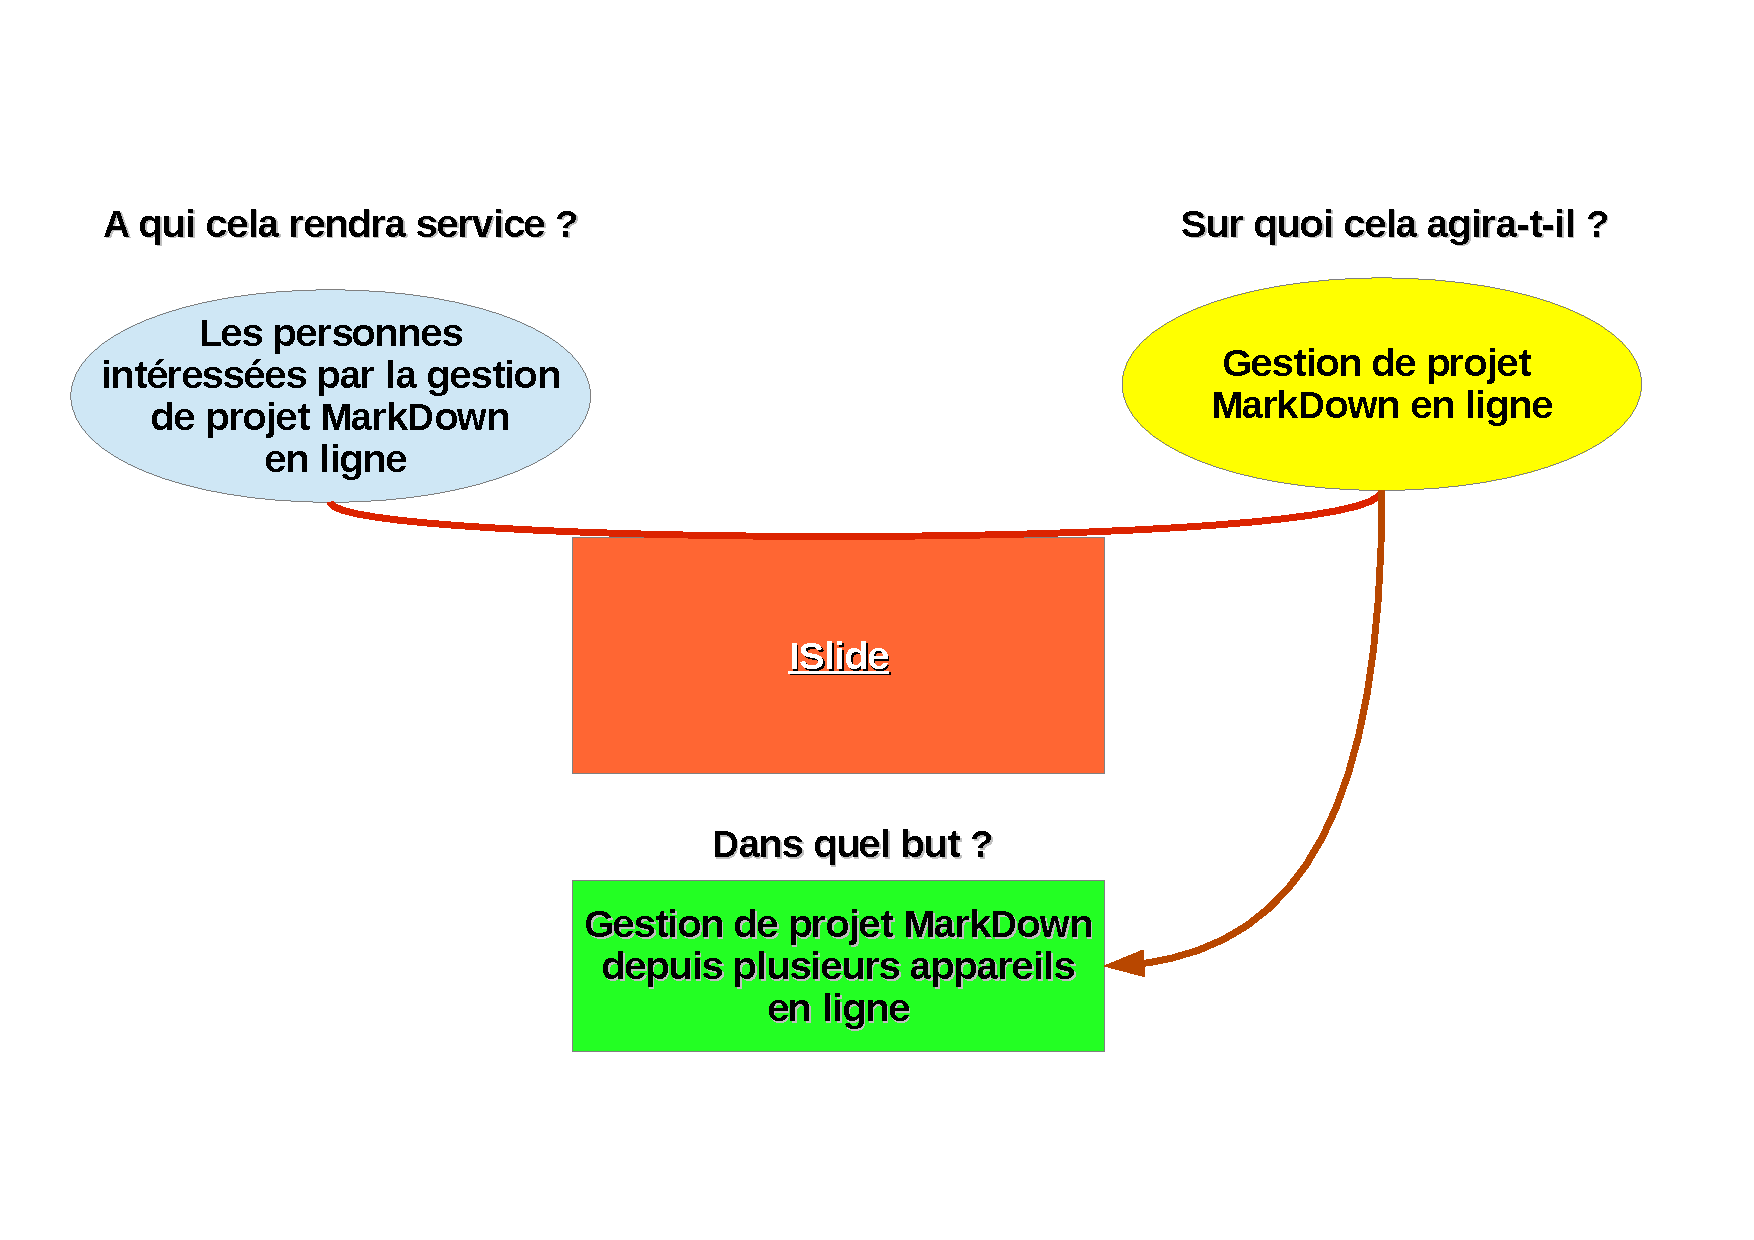
\includegraphics[scale=0.5]{bete-a-corne.pdf}


\end{document}